\documentclass{article}

\usepackage{lipsum}
\usepackage{amsfonts}
\usepackage{amsmath}
\usepackage{amsthm}
\usepackage{graphicx}
\usepackage{epstopdf}
\usepackage{algorithmic}
\ifpdf%
  \DeclareGraphicsExtensions{.eps,.pdf,.png,.jpg}
\else
  \DeclareGraphicsExtensions{.eps}
\fi
\usepackage{amsopn}
\DeclareMathOperator{\diag}{diag}
\usepackage{booktabs}
\usepackage{bbm}
\usepackage{bm}
\usepackage{caption}
\usepackage{subcaption}
\usepackage[utf8]{inputenc}
\usepackage[T1]{fontenc}
\usepackage[margin=1.5in]{geometry}
\usepackage{hyperref}

\newcommand{\norm}[1]{\left\lVert#1\right\rVert}
\newcommand{\normtwo}[1]{\left\lVert#1\right\rVert_2}
\newcommand{\abs}[1]{\left\lvert#1\right\rvert}
\newcommand{\mat}[1]{\bm{{#1}}}
\renewcommand{\vec}[1]{\bm{{#1}}}
\newcommand{\lequiv}{\Leftrightarrow}
\newcommand{\bigO}[1]{\mathcal{O}\!\left(#1\right)}
\newcommand{\ceil}[1]{\left\lceil #1 \right\rceil}
\newcommand{\floor}[1]{\left\lfloor #1 \right\rfloor}
\newcommand{\sfrac}[2]{#1/#2}
\newcommand{\hquad}{\enskip}
\newcommand{\expected}[1]{\mathbb{E}\left[#1\right]}
\newcommand{\mspan}[1]{\text{span}\left( #1 \right)}
\newcommand{\prob}[1]{P\left(#1\right)}
\newcommand{\probt}[1]{P\left( \text{#1} \right)}
\newcommand{\condprob}[2]{P\left(#1 \:|\: #2\right)}
\newcommand{\condprobt}[2]{P\left(\text{#1} \:|\: \text{#2}\right)}
\newcommand{\bayes}[2]{\frac{\condprob{#2}{#1}\prob{#1}}{\prob{#2}}}
\newcommand{\bayesx}[3]{\frac{\condprob{#2}{#1}\prob{#1}}{\condprob{#2}{#1}\prob{#1} + \condprob{#2}{#3}\prob{#3}}}
\newcommand{\sech}{\text{sech}}
\newcommand*{\vertbar}{\rule[-1ex]{0.5pt}{2.5ex}}
\newcommand*{\horzbar}{\rule[.5ex]{2.5ex}{0.5pt}}
\newcommand{\vect}[2]{\underline{{#1}}_{{#2}}}
\newcommand{\basisp}[1]{\underline{{p}}_{{#1}}}
\newcommand{\basisq}[1]{\underline{{q}}_{{#1}}}
\newcommand{\coeff}[1]{\underline{{a}}_{{#1}}}
\newcommand{\bestfit}{\underline{\bar{x}}}
\newcommand{\grad}{\nabla}
\newcommand{\laplace}{\Delta}
\newcommand{\setbar}{\:\middle|\:}
\renewcommand{\div}{\grad \cdot}
\renewcommand{\Re}{\text{Re}}

\begin{document}

\section{Setup}
The problem being solved is the rotated anisotropic diffusion equation in 2D,
\begin{equation}
  -\left(\text{div } \mat{Q}\mat{A}\mat{Q}^T\right) \grad^2 \vec{u} = 0,
\end{equation}
where $\mat{Q}$ is a rotation matrix encoding some rotation by $\theta$, and $\mat{A}$ is a diagonal
scaling matrix given by
\begin{equation}
  \mat{A} = \begin{bmatrix} 1 & 0 \\ 0 & \epsilon \end{bmatrix}.
\end{equation}

A basic training set of 100 structured $15 \times 15$ grids was constructed using a finite-element discretization.  Values of $\theta$ and $\epsilon$ were uniformly chosen within the ranges $\left[1,5\right)$ and $\left[0,\pi\right)$, respectively.  For rough testing, all figures and tables below are evaluted on a mesh with coefficients $\theta=\frac{\pi}{4}, \epsilon=3$.

    A TagConv network consisting of 5 convolutional layers was trained to predict optimal C/F partitioning. The unsupervised loss used consisted of a linear combination of the spectral radius of the multigrid error propagation operator and the 1 norm of the C/F partitioning that was output,
    \begin{equation}
      \ell\left(\vec{c}\right) := \rho\left(\mat{E}\left(\vec{c}\right)\right) + \alpha \norm{\vec{c}}_1,
    \end{equation}
    where $\mat{E}$ is defined as the error propagation for a two-level V-cycle multigrid method with using weighted Jacobi ($\omega=\frac{2}{3}$) relaxation,
    \begin{equation}
      \mat{E} := \left(\mat{I} - \omega\mat{D}^{-1}\mat{A}\right) \left(\mat{I} - \mat{P}\left(\mat{P}^T\mat{A}\mat{P}\right)^{-1}\mat{P}^T\mat{A}\right) \left(\mat{I} - \omega\mat{D}^{-1}\mat{A}\right),
    \end{equation}
    and $\mat{P}$ is the operator obtained by Ruge-St\"uben style interpolation on the C/F partitioning.
\section{Results}

\begin{figure}[h]
  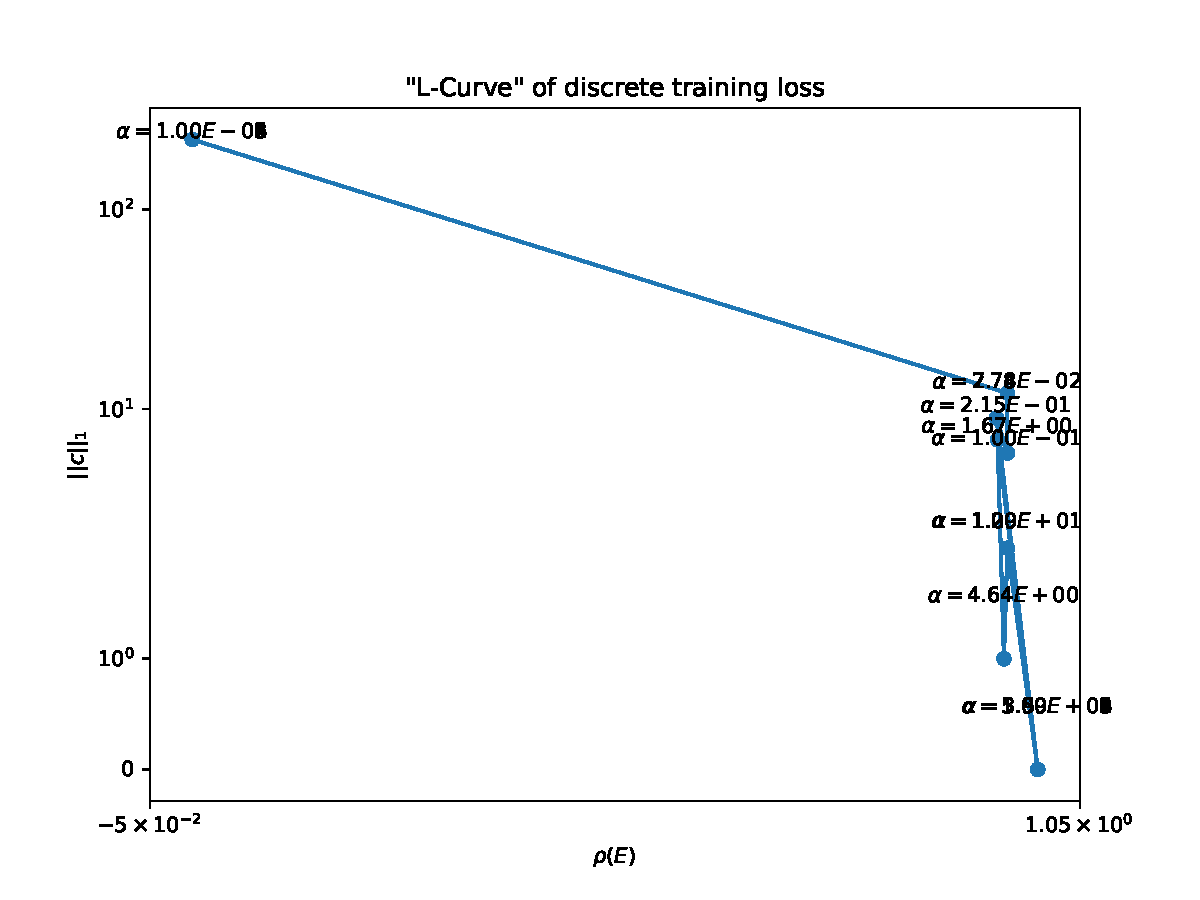
\includegraphics[width=\textwidth]{figures/lcurve.pdf}
  \caption{L-curve of $\rho\left(\mat{E}\right)$ vs $\norm{\vec{c}}_1$.  This is using a swe\,ep of $\alpha$ values between $10^{-6}$ and $10^{6}$.}
  \label{fig:lcurve}
\end{figure}

\begin{table}[h]
  \center
  \begin{tabular}{|r|r|r|r|}
    \hline
    $\alpha$ & $\rho\left(\mat{E}\right)$ & $\norm{\vec{c}}_1$ & f-fraction \\
    \hline
$1.000e-06$ & $-3.223e-16$ & $225$ & $0.000$ \\
$1.000e-05$ & $-3.223e-16$ & $225$ & $0.000$ \\
$1.000e-04$ & $-3.223e-16$ & $225$ & $0.000$ \\
$1.000e-03$ & $-3.223e-16$ & $225$ & $0.000$ \\
$1.000e-02$ & $-3.223e-16$ & $225$ & $0.000$ \\
$2.783e-02$ & $9.641e-01$ & $12$ & $0.947$ \\
$7.743e-02$ & $9.641e-01$ & $12$ & $0.947$ \\
$1.000e-01$ & $9.642e-01$ & $6$ & $0.973$ \\
$2.154e-01$ & $9.512e-01$ & $9$ & $0.960$ \\
$5.995e-01$ &  & $0$ & $1.000$ \\
$1.000e+00$ &  & $0$ & $1.000$ \\
$1.668e+00$ & $9.525e-01$ & $7$ & $0.969$ \\
$4.642e+00$ & $9.600e-01$ & $1$ & $0.996$ \\
$1.000e+01$ & $9.642e-01$ & $2$ & $0.991$ \\
$1.292e+01$ & $9.642e-01$ & $2$ & $0.991$ \\
$3.594e+01$ &  & $0$ & $1.000$ \\
$1.000e+02$ &  & $0$ & $1.000$ \\
$1.000e+03$ &  & $0$ & $1.000$ \\
$1.000e+04$ &  & $0$ & $1.000$ \\
$1.000e+05$ &  & $0$ & $1.000$ \\
$1.000e+06$ &  & $0$ & $1.000$ \\
\hline
  \end{tabular}
  \caption{Spectral radius of error propagator, norm of C/F partitioning, and f-fraction for various values of $\alpha$.}
  \label{tab:values}
\end{table}

\begin{figure}[h]
  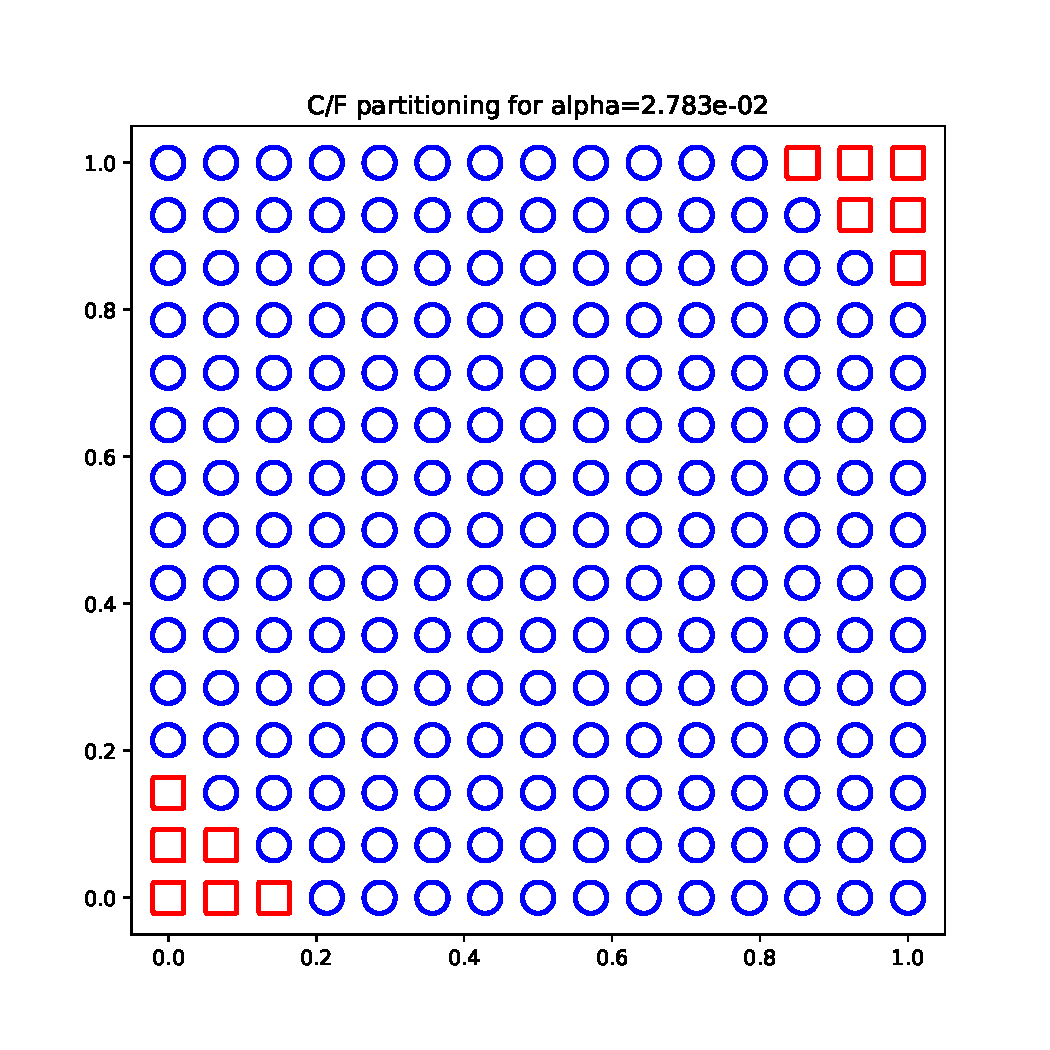
\includegraphics[width=\textwidth]{figures/cf_5.pdf}
\end{figure}

\begin{figure}[h]
  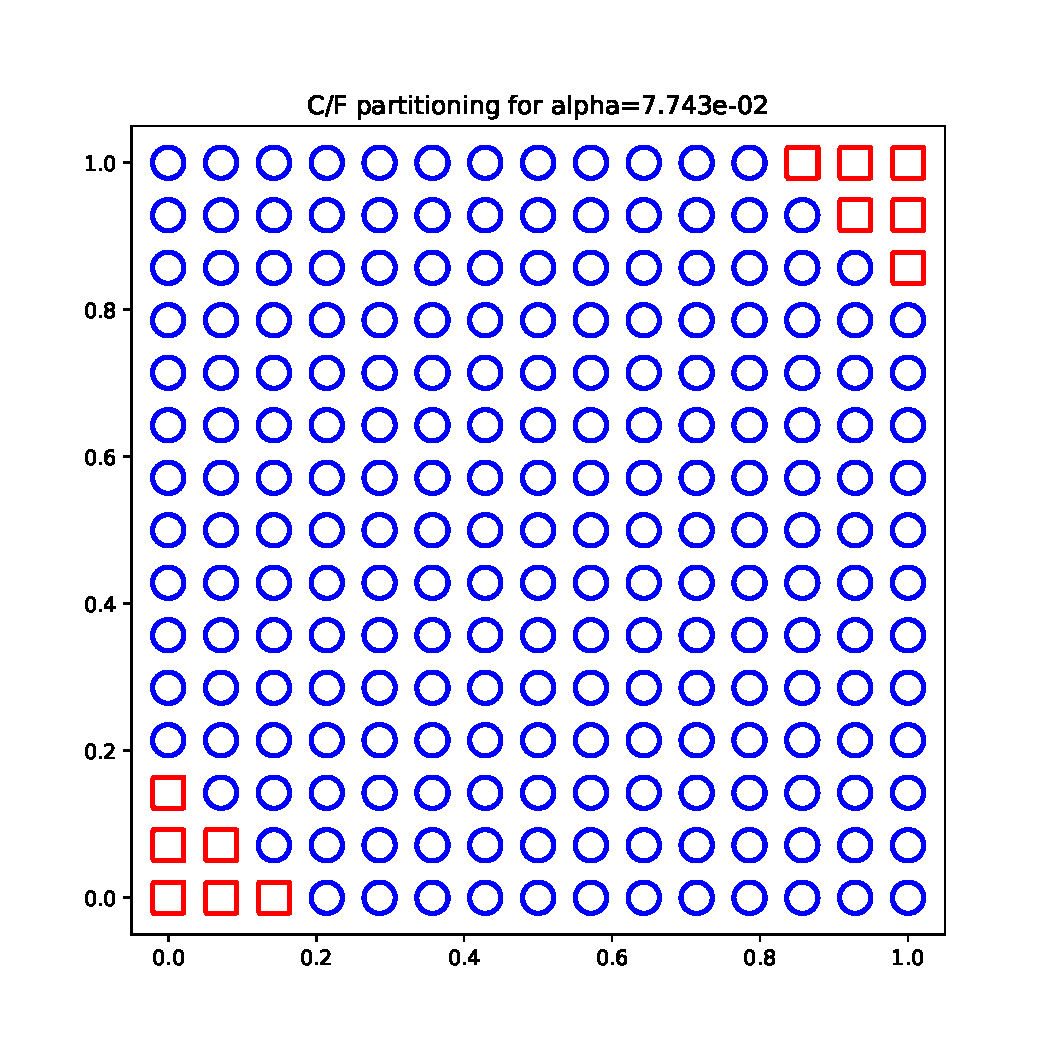
\includegraphics[width=\textwidth]{figures/cf_6.pdf}
\end{figure}

\begin{figure}[h]
  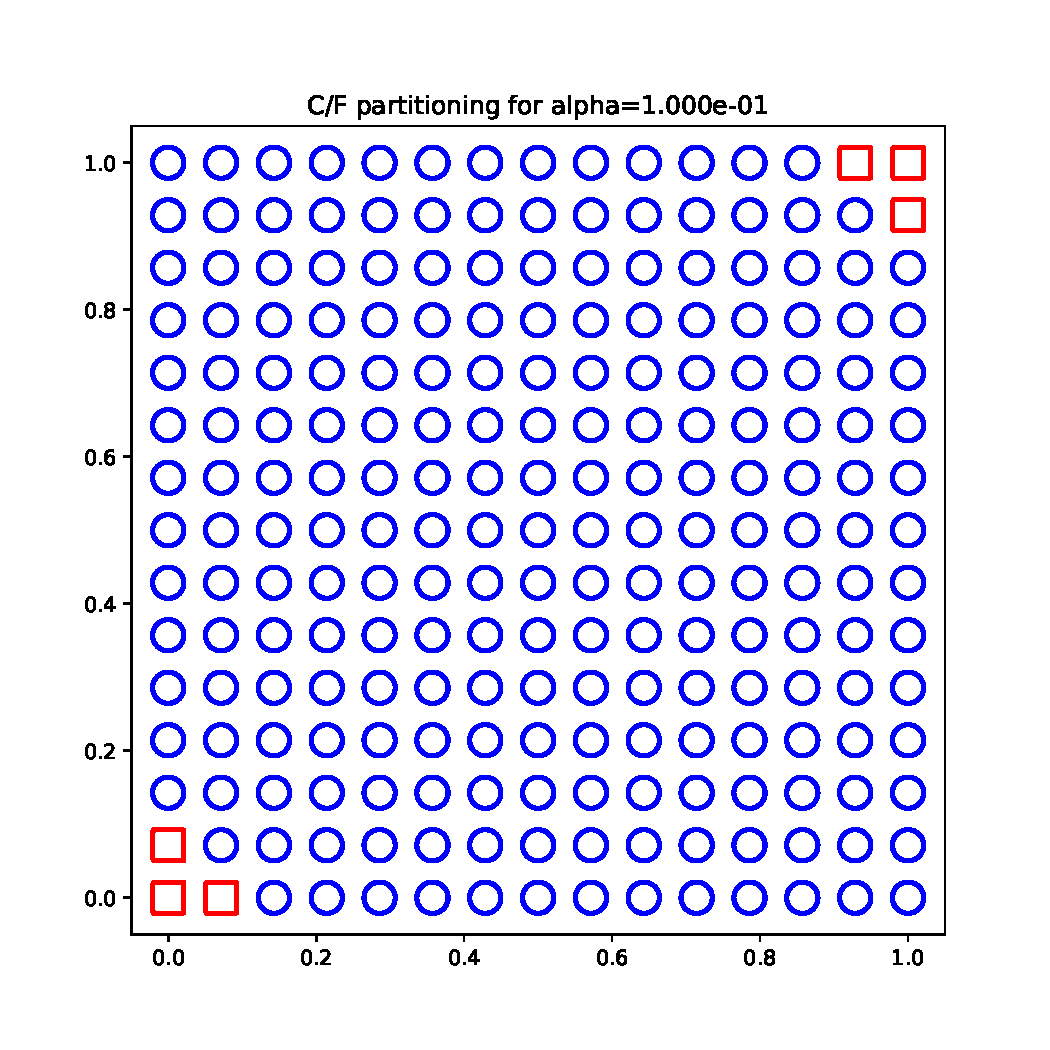
\includegraphics[width=\textwidth]{figures/cf_7.pdf}
\end{figure}

\begin{figure}[h]
  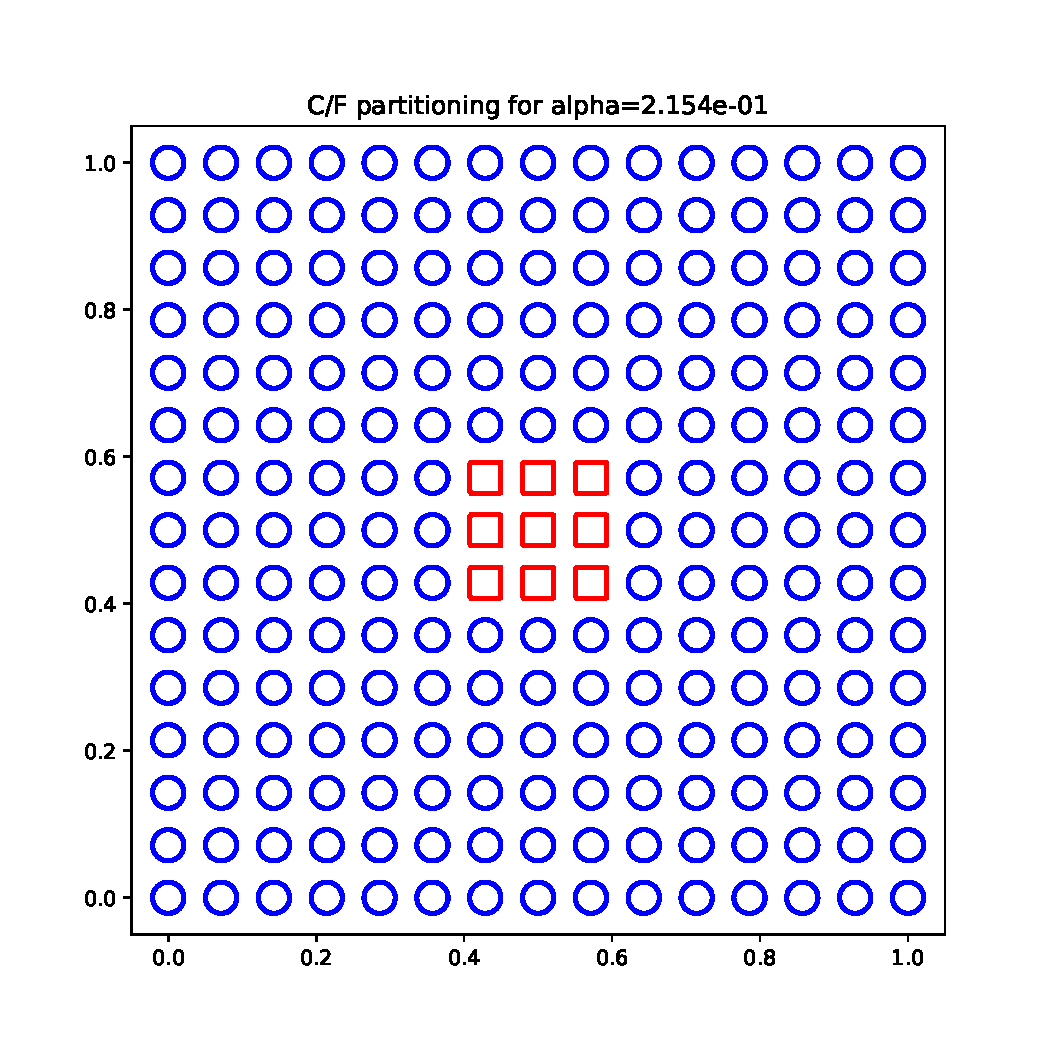
\includegraphics[width=\textwidth]{figures/cf_8.pdf}
\end{figure}

\begin{figure}[h]
  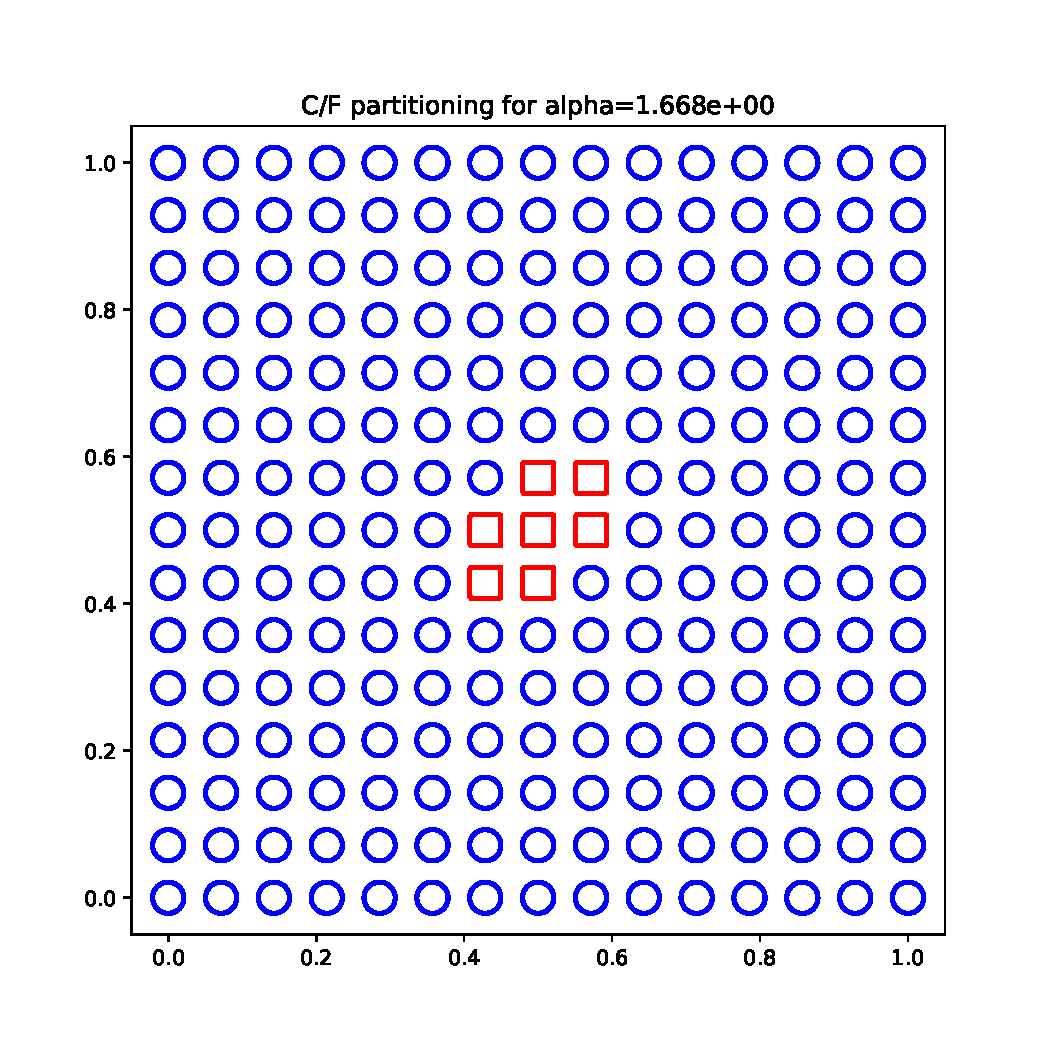
\includegraphics[width=\textwidth]{figures/cf_11.pdf}
\end{figure}

\begin{figure}[h]
  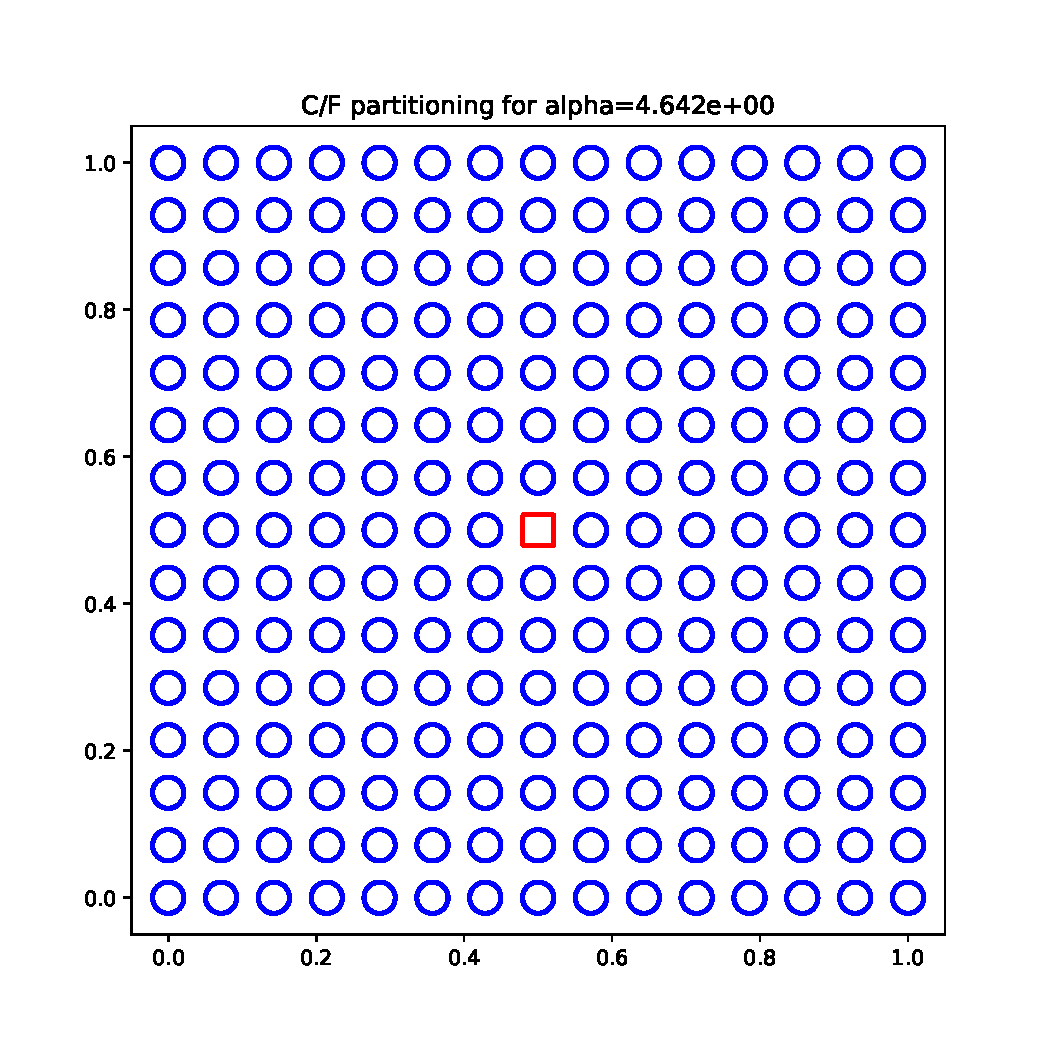
\includegraphics[width=\textwidth]{figures/cf_12.pdf}
\end{figure}

\begin{figure}[h]
  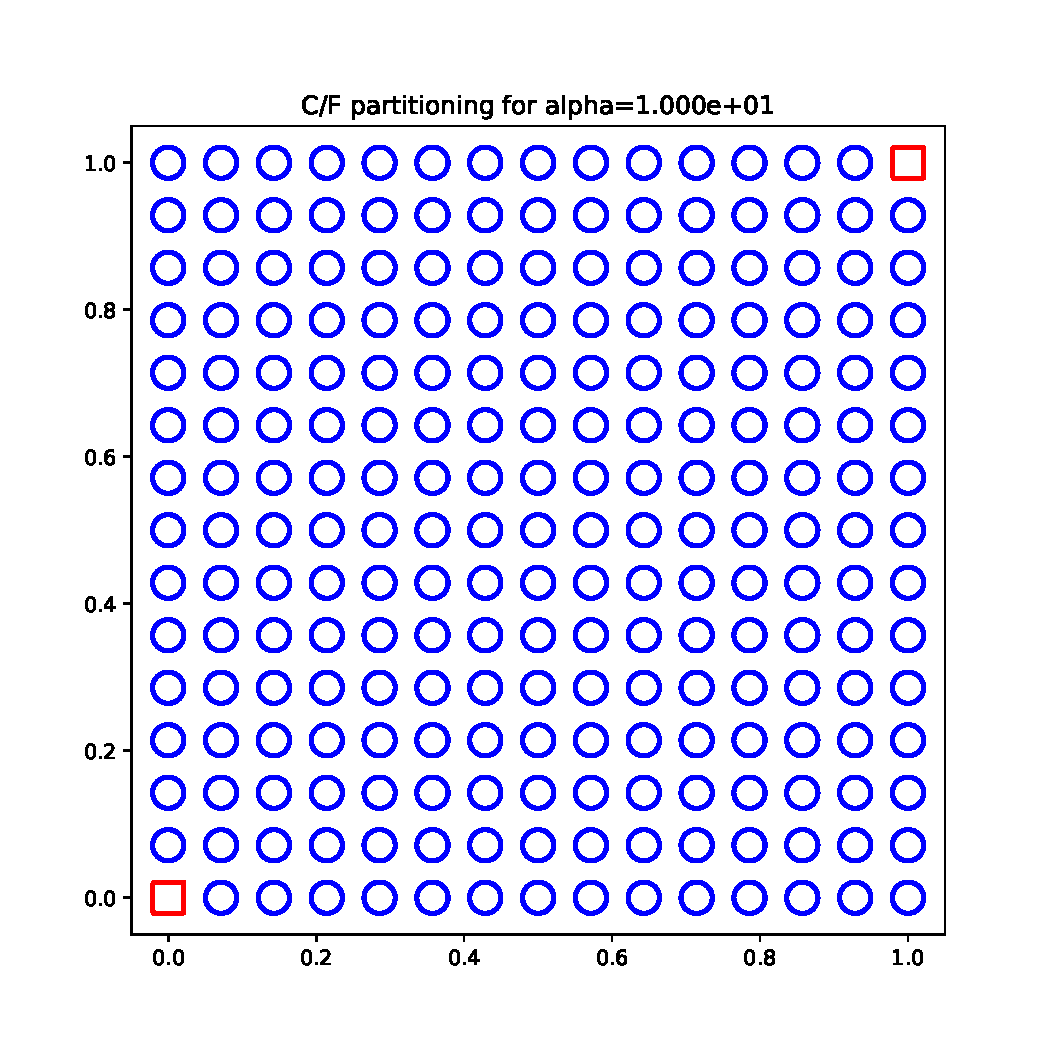
\includegraphics[width=\textwidth]{figures/cf_13.pdf}
\end{figure}

\begin{figure}[h]
  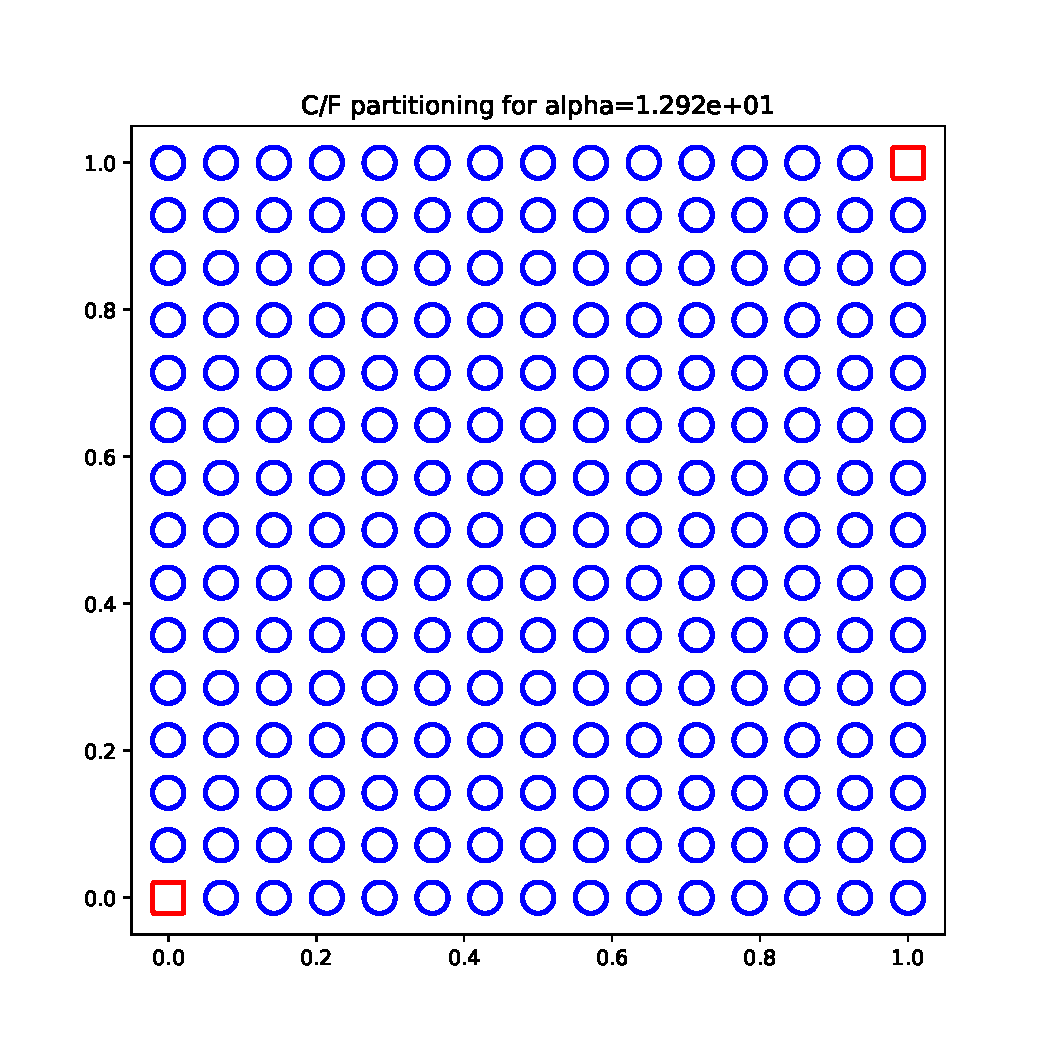
\includegraphics[width=\textwidth]{figures/cf_14.pdf}
\end{figure}

\end{document}
